\documentclass{beamer}
\usetheme{Madrid}
\usecolortheme{default}
\newcommand{\standardlogo}{%
  \hfill
  \raisebox{0pt}[0pt][0pt]{%
    %
\includegraphics[height=1cm]{figures/CSGSU_logo.png}\hspace{6pt}%
    
\includegraphics[height=0.5cm]{figures/TMU-rgb}%
  }%
}
\newcommand{\titlelogo}{%
  \hfill
  \raisebox{0pt}[0pt][0pt]{%
    %\raisebox{-5pt}{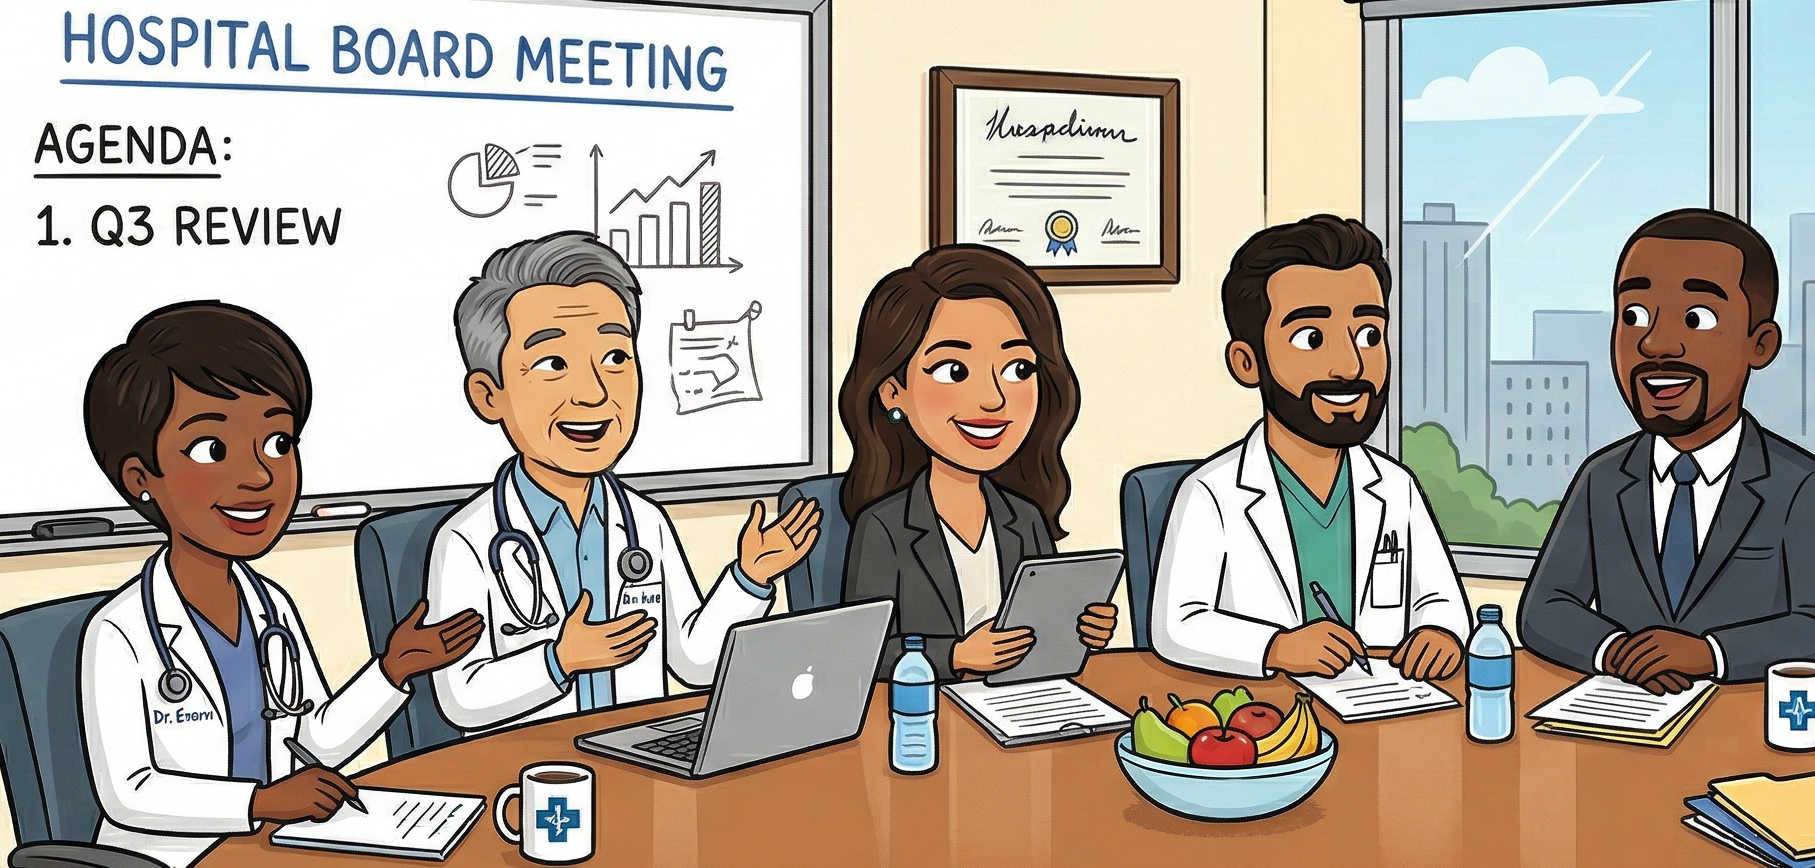
\includegraphics[height=3cm]{figures/Gemini_Generated_Image_rz8xj0rz8xj0rz8x.png}\hspace{200pt}}%
    % 
\includegraphics[height=1cm]{figures/CSGSU_logo.png}\hspace{6pt}%
    \raisebox{4pt}{
\includegraphics[height=0.9cm]{figures/TMU-rgb}}%
  }%
}
\setbeamertemplate{logo}{\standardlogo}
\newcommand{\nologo}{\setbeamertemplate{logo}{}}
\definecolor{TMU_blue}{RGB}{35,79,149}
\setbeamercolor{titlelike}{bg=TMU_blue}
\setbeamerfont{title}{size=\Huge,series=\bfseries}
\setbeamercolor{section number projected}{bg=TMU_blue}
\usepackage{multirow}
\usepackage{graphicx}
\usepackage{forest}
\usepackage{filecontents}
%\usepackage{enumitem}
\usepackage{booktabs}
\usepackage{makecell}
\usepackage[table]{xcolor}
\usepackage{pgfplots}

\usepackage{tikz}
\usetikzlibrary{positioning,arrows.meta,shapes.geometric,calc}
\usepackage{fontawesome5}

\usepackage{array}
\newcolumntype{C}[1]{>{\centering\let\newline\\\arraybackslash\hspace{0pt}}m{#1}}

% Optional bibliography support (not used in this deck)
\usepackage[style=authoryear-icomp,autocite=footnote,maxnames=1,babel=hyphen,hyperref=true,abbreviate=true,backend=biber,mcite]{biblatex}
\addbibresource{slides.bib}

% Section TOC
\AtBeginSection[]
{
  \begin{frame}
    \frametitle{Table of Contents}
    \hfill
    \parbox[t]{0.95\textwidth}{
    \begin{minipage}[c][0.7\textheight]{\textwidth}
    \tableofcontents[currentsection]
    \end{minipage}
    }
  \end{frame}
}

% TITLE SLIDE ------------------------------------------------
\title[CP8305 (Knowledge Discovery)]{Unmasking Readmission}
\subtitle{Cost-Sensitive, Transparent Knowledge Discovery for 30-Day
Hospital Readmission in Diabetic Patients}

\author[Group Name]{%
  Christopher Indris \and Mojtaba Mohammadi \and Mohammad Al Batayneh
}

\institute[TMU]{Toronto Metropolitan University \\ CP8305 - Knowledge Discovery}
\date[April 10th, 2026]{April 10th, 2026}

\begin{document}
\setbeamertemplate{logo}{\titlelogo}
\frame{\titlepage}
\setbeamertemplate{logo}{\standardlogo}

% ==========================================================
\section{Introduction}

\begin{frame}\frametitle{Problem and Goal}
\begin{itemize}
    \item \textbf{Industry Challenge:} Inability to predict short-term patient readmissions leads to:
    \begin{itemize}
      \item Misdiagnosed severity
      \item Suboptimal resource allocation
      \item Financial penalties under HRRP\footcite{strack_impact_2014}
    \end{itemize}
    \vspace{6pt}
    \item \textbf{Project Goal:} Predictive and Perscriptive analysis of 30-day readmission risk in diabetic patients
    \begin{itemize}
      \item Transparent methods, for trust
    \end{itemize}
    \vspace{6pt}
    \item \textbf{Expected Impact:} 
    \begin{itemize}
      \item Methods which are both interpretable and performative
      \item Actionable insights for decision-making
    \end{itemize}
\end{itemize}
\end{frame}

% ==========================================================
\section{Data Strategy \& Exploration}

\begin{frame}\frametitle{Task Overview}
\begin{itemize}
    \item \textbf{Source:} Diabetes 130-US Hospitals dataset (1999-2008), Cerner Health Facts.
    \vspace{4pt}
    \item \textbf{Target Variable Formulation:} Binary classification aligning with HRRP penalty windows:
    \begin{itemize}
      \item \textbf{Positive (High-Risk):} $<30$ days readmission (Minority class: ~11\%)
      \item \textbf{Negative (Low-Risk):} $>30$ days or NO readmission
    \end{itemize}
    \vspace{4pt}
\end{itemize}
\end{frame}

\begin{frame}\frametitle{Challenges}
\begin{itemize}
    \item \textbf{Identified Gaps to Address:}
    \begin{itemize}
        \item ``Black-box'' ensemble models (e.g., XGBoost) lack the clinical transparency required for actionable healthcare decisions.
    \end{itemize}
    \vspace{6pt}
    \item \textbf{Data Manipulation Hurdles:}
    \begin{itemize}
        \item \textbf{Class Imbalance:} Only ~11\% of records for the readmission case.
        \item \textbf{Sparsity:} Many missing, non-estimatable values
        \item \textbf{High Cardinality:} 100's of medical codes; domain knowledge to combine.
        \item \textbf{Leaky Variables:} Patient codes non-unique; some discharges indicate mortality.
    \end{itemize}
\end{itemize}
\end{frame}

\begin{frame}\frametitle{Limitations of Prior Work}
\begin{itemize}
    \item \textbf{Existing Research Lacks:}
    \begin{itemize}
        \item punishment of false negatives \footcite{rubin_correction_2018}
        \item inpatient vs. outpatient medications \footcite{rubin_correction_2018}
        \item focus on transparent models \footcite{liu_comparison_2024}
        \item production of rule sets for clinical use \footcite{liu_comparison_2024}
    \end{itemize}
\end{itemize}
\end{frame}

% ==========================================================
\section{Methodology: Preprocessing \& Modeling}

\begin{frame}\frametitle{Data Preprocessing Pipeline}
\begin{itemize}
    \item \textbf{Feature Engineering:} Proposing new clinical variables.
    \vspace{6pt}
    \item \textbf{Addressing Imbalance:} Accurately model the minority class via:
    \begin{itemize}
      \item SMOTE
      \item Cost-Sensitive Reweighting
    \end{itemize}
\end{itemize}
\end{frame}

\begin{frame}\frametitle{Modeling: Interpretability vs. Performance}
\begin{itemize}
    \item \textbf{Our Approach:} Benchmark top models and interpretable, rule-based algorithms.
    \vspace{6pt}
    \item \textbf{Candidate Models/Systems:}
    \begin{itemize}
        \item \textit{Transparent Base:} Logistic Regression, Decision Trees.
        \item \textit{Rule-Induction:} PRISM / Association Rules (human-readable logic).
        \item \textit{Black-Box Top Performer:} XGBoost.
        \item \textit{SHAP:} for black-box model interpretation.
    \end{itemize}
\end{itemize}
\end{frame}

% ==========================================================
\section{Cost-Sensitive Evaluation Framework}

\begin{frame}\frametitle{Why Accuracy Isn't Enough}
\begin{itemize}
    \item \textbf{Metrics/Systems:}
    \begin{itemize}
      \item \textit{Stratified CV:} avoid leakage.
      \item \textit{AUPRC:} for rare events
      \item \textit{Kappa:} for dataset skew
      \item \textit{Brier Score:} for true clinical likelihood
    \end{itemize}
\end{itemize}
\end{frame}

\begin{frame}\frametitle{The Cost-Sensitive Framework}
\begin{itemize}
    \item \textbf{False Negative (Missed High-Risk):} High Cost. Patient readmits within 30 days, triggering heavy HRRP financial penalties and resource strain.
    \vspace{6pt}
    \item \textbf{False Positive (Unnecessary Intervention):} Low-to-Moderate Cost. Enrolling a patient in preventive care (e.g., follow-up calls) who wouldn't have readmitted.
    \vspace{6pt}
    \item \textbf{Goal:} Optimize the threshold to minimize overall financial and operational cost, not just classification error.
\end{itemize}
\end{frame}

% ==========================================================
\section{Findings \& Recommendations}

\begin{frame}\frametitle{Initial Scores (Without the Tricks)}

\begin{center}
  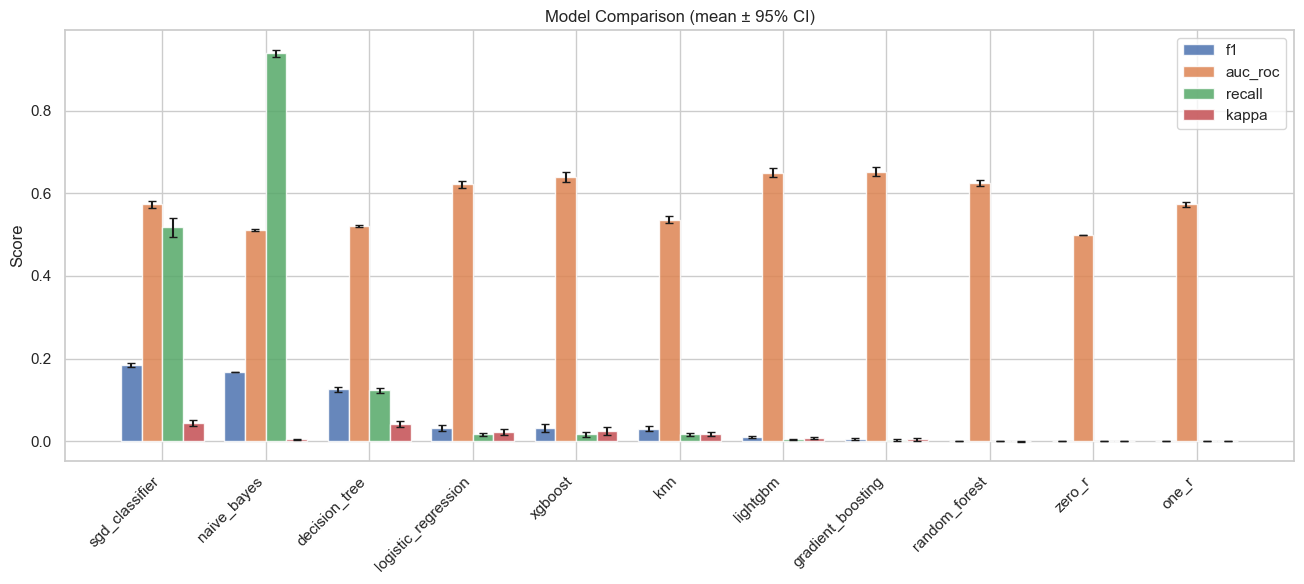
\includegraphics[height=5.5cm]{figures/performance.png}
\end{center}

\begin{itemize}
    \item Dataset imbalance is a significant challenge; AUC-ROC handles the class imbalance best. This shows the importance of attribute elimination and identifying the classes correlating with the target. 
\end{itemize}
\end{frame}

\begin{frame}\frametitle{Initial Insights \& Business Value}
\begin{itemize}
    \item \textbf{Clinical Application:} Transitioning from ``black-box scoring'' to transparent risk triggers enables targeted preventive resource allocation at discharge.
    \vspace{6pt}
    \item \textbf{Recommendation:} Deploy an interpretable rule-set overlay to flag high-risk discharges, balancing intervention costs against HRRP penalty risks.
\end{itemize}
\end{frame}

% ==========================================================
\section{Conclusion}

\begin{frame}\frametitle{Conclusion \& Next Steps}
\begin{itemize}
    \item \textbf{Summary:} Shifted focus from raw prediction to Cost-Sensitive Knowledge Discovery, providing interpretable rules to mitigate HRRP readmission penalties.
    \begin{itemize}
      \item Focus: raw prediction to cost-sensitive discovery
      \item Provide interpretable rules for clinicians
    \end{itemize}
    \vspace{6pt}
    \item \textbf{Next Steps in Analysis:} 
    \begin{itemize}
      \item Whittle away at the attributes for better fit and interpretability.
    \end{itemize}
\end{itemize}
\end{frame}

\begin{frame}\frametitle{Thank You!}
\begin{center}
  \vspace{10pt}
  \textbf{Questions?}
  \vspace{20pt}
  
  \textit{Project Repository: github.com/chrisindris/CP8305FP}

  \vspace{20pt}
  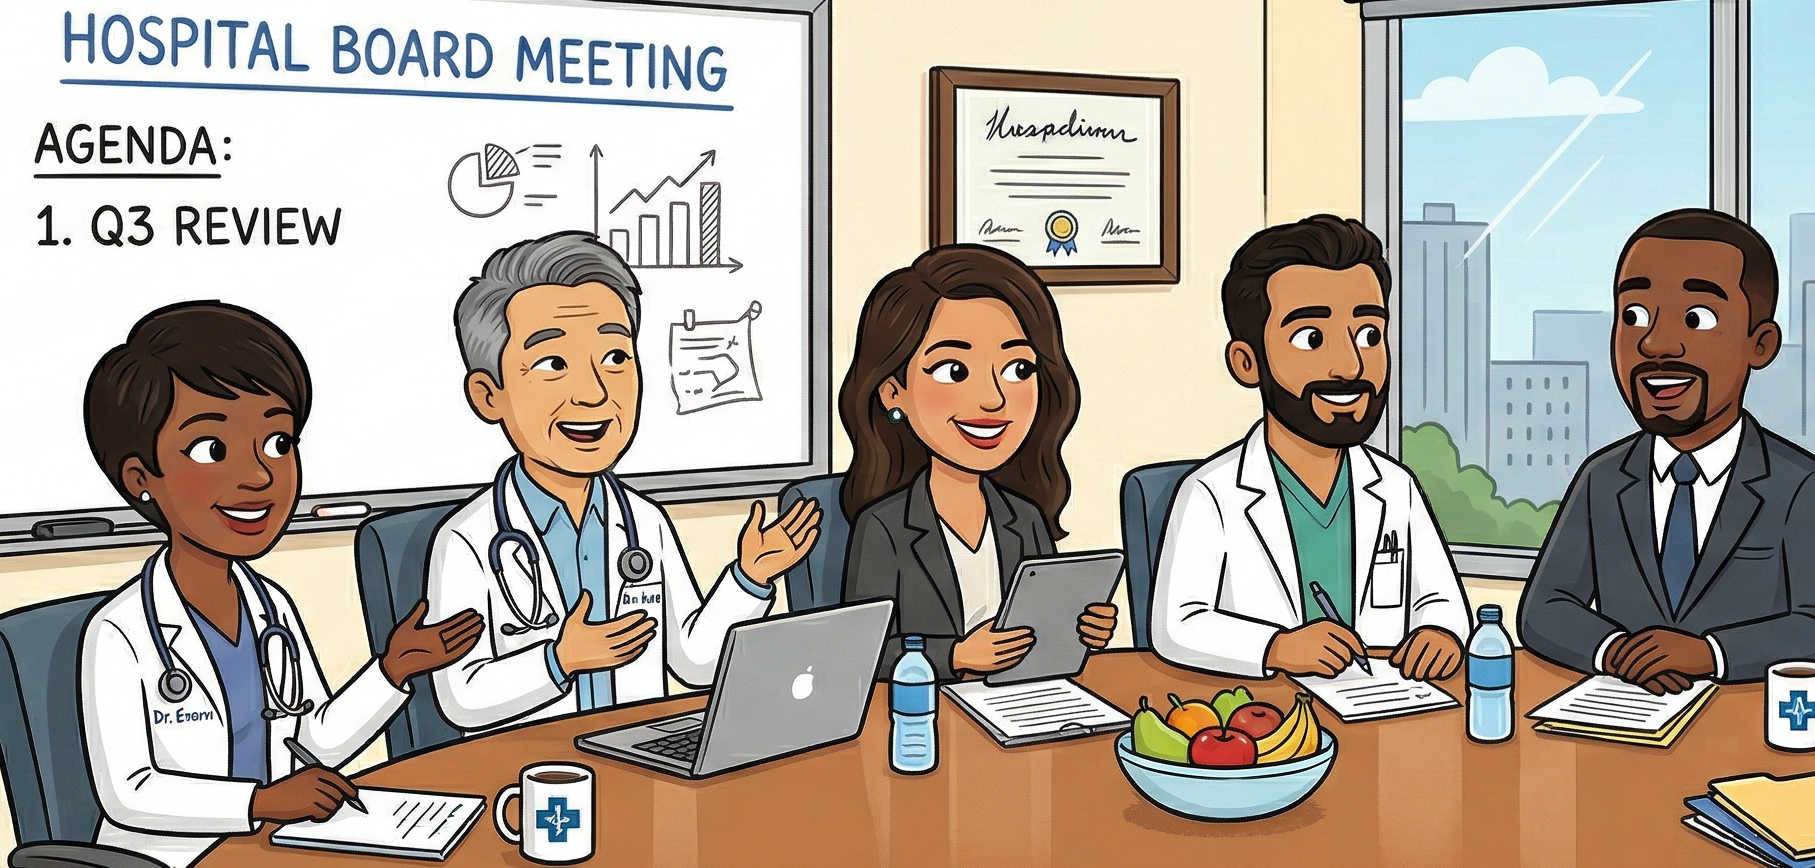
\includegraphics[height=3cm]{figures/Gemini_Generated_Image_rz8xj0rz8xj0rz8x.png}

\end{center}
\end{frame}

\end{document}
